\section{Определение комплексного
числа}\label{ux43eux43fux440ux435ux434ux435ux43bux435ux43dux438ux435-ux43aux43eux43cux43fux43bux435ux43aux441ux43dux43eux433ux43e-ux447ux438ux441ux43bux430}

\textbf{Определение:} \emph{Комплексными числами} называются пары
\((x,y)\) действительных чисел \(x\) и \(y\), если для них определены
понятия равенства и операции сложения и умножения следующим образом:

\begin{enumerate}
\def\labelenumi{\arabic{enumi}.}
\tightlist
\item
  Два комплексных числа \((x_{1},y_{1})\) и \((x_{2},y_{2})\) считаются
  \emph{равными} тогда и только тогда, когда \(x_{1}=x_{2}\) и
  \(y_{1}=y_{2}\).
\item
  \emph{Суммой} двух комплексных чисел \((x_{1},y_{1})\) и
  \((x_{2},y_{2})\) называется комплексное число
  \((x_{1}+x_{2},y_{1}+y_{2})\).
\item
  \emph{Произведением} двух комплексных чисел \((x_{1},y_{1})\) и
  \((x_{2},y_{2})\) называется комплексное число
  \((x_{1}x_{2}-y_{1}y_{2},x_{1}y_{2}+x_{2}y_{1})\).
\end{enumerate}

Формулы: \[
(x_{1},y_{1})=(x_{2},y_{2})\text{, если } x_{1}=x_{2}\text{ и }y_{1}=y_{2}\quad(1)
\] \[
(x_{1},y_{1})+(x_{2},y_{2})=(x_{1}+x_{2},y_{1}+y_{2})\quad(2)
\] \[
(x_{1},y_{1})\cdot(x_{2},y_{2})=(x_{1}x_{2}-y_{1}y_{2},x_{1}y_{2}+x_{2}y_{1})\quad(3)
\]

\textbf{Определение:} Множество комплексных чисел, в котором введено
равенство, а также операции сложения и умножения, обозначают
\(\mathbb{C}\).

\textbf{Определение:} Комплексное число \((0,1)\) называют \emph{мнимой
единицей} и обозначается буквой \(i\). По формуле (3): \[
i^{2}=(0,1)\cdot(0,1)=(-1,0)=-1
\] Тогда по формулам (2) и (3): \[
(x,y)=(x,0)+(0,1)(y,0)=x+iy
\] Комплексные числа можно записать в алгебраической форме: \[
(x,y)=x+iy
\]

\textbf{Определение:} Комплексные числа вида \(0+iy\) называют
\emph{чисто мнимыми}.

Комплексное число \(x+iy\) принято обозначать одной буквой \(z\), т.е.
\(z=x+iy\). Число \(x\) называется \emph{действительной частью}, а число
\(y\) - \emph{мнимой частью} комплексного числа \(z=x+iy\). Для этих
чисел приняты следующие обозначения: \[
x=\mathrm{Re}(x+iy)=\mathrm{Re}z\quad y=\mathrm{Im}(x+iy)=\mathrm{Im}z
\]

\textbf{Определение:} Комплексное число \(x-iy\) называется
\emph{сопряженным} с комплексным числом \(z=x+iy\) и обозначается
\(\overline{z}\), т.е. \[
\overline{z}=\overline{x+iy}=x-iy
\]

\textbf{Определение:} Число \(\sqrt{ x^{2}+y^{2} }\) называется
\emph{модулем} комплексного числа \(z=x+iy\) и обозначается \(|z|\),
т.е. \[
|z|= |x+iy|=\sqrt{ x^{2}+y^{2} }
\] Соответствие между комплексными числами и точками плоскости является
взаимно однозначным. При этом действительные числа изображаются точками
оси абсцисс, а чисто мнимые --- точками оси ординат. Поэтому ось абсцисс
называется \emph{действительной осью}, а ось ординат - \emph{мнимой
осью}. Плоскость, на которой изображаются комплексные числа, называется
\emph{комплексной плоскостью}.

\textbf{Формы записей:}

\begin{enumerate}
\def\labelenumi{\arabic{enumi}.}
\tightlist
\item
  \(z=x+iy\) - алгебраическая
\item
  \(z=r(\cos \varphi+i\sin\varphi)\) - тригонометрическая,
\item
  \(z=re^{ i\varphi }\) - показательная, где \(r=|z|\), а
  \(\varphi=\arg z\) - угол между вектором \(z\) и положительным
  направлением действительной оси.
\end{enumerate}

\pandocbounded{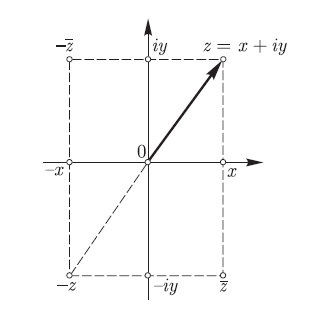
\includegraphics[keepaspectratio]{Вопросы/media/Pasted image 20260605151104.png}}
